\section{Gestion des mati{\`e}res}

\begin{center}
\scalebox{0.7}{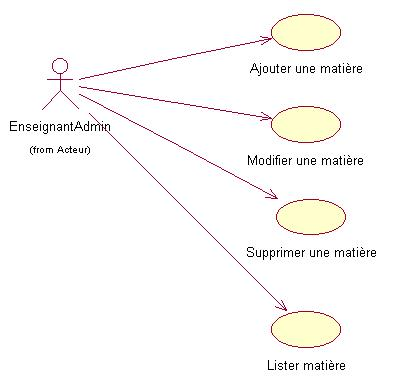
\includegraphics{images/matiere.jpg}}\\
\par{Package Gestion Matiere}
\end{center}
Voici les diff{\'e}rents sc{\'e}narios:\\

\section*{EnseignantAdmin}

\begin{tabular}{|p{4cm}|c|p{4cm}|p{5cm}|}
\hline
  Fonction & Priorit{\'e} & Qualit{\'e} & Mesure \\
\hline
cr{\'e}er une mati{\`e}re & 4 & Fiable, Facile & Pas de redondance. Ergonomique.\\
\hline
Modifier une mati{\`e}re & 2 & Fiable, Facile & Coh{\'e}rence avec les
  enseignements. Ergonomique.\\
\hline
Supprimer une mati{\`e}re & 4 & Fiable & Archivage. \\
\hline
Lister les mati{\`e}res & 4 & Rapide et Complet & Permettre de lister
  rapidement les mati{\`e}res existantes et assurer le
  listing de toutes les mati{\`e}res sans en oublier.\\
\hline
\end{tabular}

\begin{center}
{\'e}chelle de mesure de la priorit{\'e}:

\scalebox{0.5}{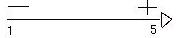
\includegraphics{images/echelle.jpg}}
\end{center}

\begin{itemize}
\item  {\bf Cr{\'e}er mati{\`e}re :}
	\begin{itemize}
	\item Pr{\'e}-requis : Etre log{\'e} 
	\item Description :Il s'identifie avec son login et son mot de passe. \\
	Il saisie la nouvelle mati{\`e}re et valide.
	\item Post-requis : Une nouvelle mati{\`e}re est cr{\'e}{\'e}e si elle n'existait pas.
	\end{itemize}

\item  {\bf Modifier mati{\`e}re :}
	\begin{itemize}
	\item Pr{\'e}-requis : Etre log{\'e} et cr{\'e}ateur de la section.
	\item Description : Il s'identifie avec son login et son mot de passe.\\
	Il selectionne la mati{\`e}re de son choix et clique l'option {\it Modification} et valide.\\
	Seul le cr{\'e}ateur de la mati{\`e}re peut la modifier.
	\item Post-requis : La mati{\`e}re est modifi{\'e}e.
	\end{itemize}

\item  {\bf Supprimer mati{\`e}re :}
	\begin{itemize}
	\item Pr{\'e}-requis : Etre log{\'e} et cr{\'e}ateur de la mati{\`e}re.
	\item Description : Il s'identifie avec son login et son mot de passe.
	Il selectionne la section de son choix et clique l'option {\it Suppression} et valide.\\
	Une fen{\^e}tre de confirmation apparait, il confirme son choix
	\item Post-requis : On archive tous les enseignements qui faisait partie de cette mati{\`e}re.
	\end{itemize}

\item  {\bf Lister les mati{\`e}res :}
	\begin{itemize}
	\item Pr{\'e}-requis : Etre log{\'e}.
	\item Description : Il s'identifie avec son login et son mot de passe.\\
	Il demande le listing des mati{\`e}res.\\
	Elles apparaissent dans une fen{\^e}tre.
	\item Post-requis : Il peut effectuer une action {\it Modification, Suppression} sur la mati{\`e}re s{\'e}lectionn{\'e}e.\\
	\end{itemize}
\end{itemize}
